% Do not change document class, margins, fonts, etc.
\documentclass[a4paper,oneside,bibliography=totoc]{scrbook}
\setlength{\parindent}{25pt}
\newtheorem{definition}{Definition} \newtheorem{proposition}{Proposition}


% Add packages
\usepackage[colorlinks=false]{hyperref}
\usepackage[utf8]{inputenc}
\usepackage{emptypage}
\usepackage{enumitem}
\usepackage{graphicx}
\graphicspath{ {./figs/} }
\usepackage[justification=raggedright]{caption}
\captionsetup{labelformat=empty, textformat=empty}
\usepackage{latexsym}
\usepackage{amsmath}
\usepackage{amssymb}
\usepackage{tabularx}
\usepackage{booktabs}
\usepackage{algorithm} % you can modify the algorithm style to your liking
\usepackage{algorithmic}
\usepackage{csquotes}
\renewcommand{\algorithmiccomment}[1]{\hfill\textit{// #1}}
\usepackage[usenames,dvipsnames]{xcolor}
\usepackage[colorlinks,citecolor=Green]{hyperref} % you may change/remove the colors
\usepackage{lipsum} % you do not need this

% Citation style
\usepackage{cite
\usepackage{csquotes}
\bibliographystyle{chicagoa}
\setcitestyle{authoryear,round,semicolon,aysep={},yysep={,}} \let\cite\citep

% ----------------------------------------------------------------------------------------------
% Begin Documents
\begin{document}

% Cover page
\frontmatter \subject{Master Thesis} % change to appropriate type
\title{\LARGE 
	Uncertainty Calibration with Online Conformal Prediction in Neural Architecture Search: \\ 
	An Evaluation under the BANANAS Framework 
}
\author{
	Cheng Chen\\ (matriculation number 1662473)} \date{July 31, 2025
}
\publishers{
	{\small Submitted to}\\
	Data and Web Science Group\\Prof.\ Dr.\ Margret Keuper\\University of Mannheim\\
}
\maketitle

% Abstract
\chapter{Abstract}
Some contents


% Table of contents
\begingroup%
\hypersetup{hidelinks} % disable link color in TOC only
\tableofcontents%
\endgroup


% List of algorithms/figures/tables
\listofalgorithms 
\listoffigures 
\listoftables


% Body
\mainmatter  % start new numbering

% chapter 1
\chapter{Introduction}
\label{ch:intro}

\section{Motivation}
\section{Related Work}
\section{Contributions and Limitations}
\section{Outline}


% chapter 2
\chapter{Literature Review}
\label{ch:related_work}

\section{Neural Architecture Search (NAS)}

\subsection{Background}
NAS is a subfield of AutoML.
\begin{description}
	\item [Search Space] Details will be introduced in \ref{Dataset}
	\item [Search Strategy] 
	\item [Performance Evaluation]
\end{description}}

\subsection{BANANAS}
\label{sec:bananas}
Bayesian Optimization with Neural Architectures for Neural Architecture Search (BANANAS)




BANANAS is an Bayesian Optimization based search strategy. 



Bayesian optimization is a sequential decision-making process that seeks to find a global minimum x⋆ ∈ argminx∈X f(x) of an unknown black-box objective function f : X → R over an input space X ⊆ RD. 





Give an introduction how Bayesian Optimization works. We list the five engineering decisions and review each field's related works. Maybe briefly cite Gaussian Process.

\begin{description}[leftmargin=0cm]
	\item [Architecture Encoding]
	\item [Neural Predictor]
	\item [Uncertainty Estimation] 
	\item [Acquisition Function]
	\item [Acquisition Optimization]
\end{description}}


\section{Uncertainty Quantification}
Understanding uncertainty is important for real-world application of artificial intelligence, e.g., in autonomous driving, medical diagnosis. 

\subsection{Types of Uncertainty}
- aleatory uncertainty (data uncertainty): uncertainty that arises due to inherent variations and randomness, and cannot be reduced by collecting more information \\
- epistemic uncertainty (model uncertainty): uncertainty that arises due to lack of knowledge, and can be reduced by collecting more information.

\subsection{Alternative Uncertainty Estimation Methods}
- Bayesian-based: e.g., Bayesian Neural Network \\
- Ensemble-based: e.g., Monte-Carlo dropout \\
- Bootstrapping \\
But these techniques are limited in several perspectives. First, quantifying uncertainty requires training models for several times, which means that the models cannot be applied for real-time prediction or in an online-learning setup. Second, some models are pre-trained and are only accessible via API. Besides, models (pre-)trained on certain datasets may struggle to generalize across different domains or contexts. 

\section{Conformal Prediction}
\label{sec: reviewCP}

\subsection{Theoretical Background}
Starting from i.i.d data, and provide an intuitive demonstration how the prediction interval is constructed (can add a figure illustrating why conformal prediction works, i.e., symmetry). From the most intuitive expression to the finite-sample adjusted expression. 
		
\begin{description}[leftmargin=0cm]
	\item [Notation] Then, relax the i.i.d assumption to exchangeability, and lay a formal definition of the conformal prediction. And list the most importance three ingredients of the conformal predictions. \\
	- A trained predictor f \\
	- A conformity score function s. The conformity score is an important engineering decision and has an impact on the size on the prediction set, i.e., the efficiency. The conformity score function can be either a negatively- or positively oriented, in which … And it can be a random variable as well. \\
	-	A target coverage alpha	\\

		Marginal coverage is guaranteed regardless of the choices in dataset and black
		box model. Only the model predictions are required to apply the technique.
	\item [A Link to Statistical Testing] (clarify the relationship between conformal prediction and hypothesis testing) In this video (22:21), it is explained the intuition why conformal prediction guarantees the coverage, which is quite similar to the spirit of hypothesis testing. 
	
	     \begin{table}[h]
    		\centering
    		\caption{Comparison between CP and Hypothesis Testing}

    		\renewcommand{\arraystretch}{1.2}
   			\begin{tabular}{| m{6cm} | m{6cm} |}
     			\hline
      		   	\textbf{CP} & \textbf{Hypothesis Testing} \\
               	\hline
        		(desired) Coverage level & Confidence level \\
        	   	\hline
        		Nominal error level (1 - Coverage level) & Significance level \\
        		\hline
        		The conformity score of the new instance & p-value (is an empirical term) \\
        		\hline
    		\end{tabular}
        	\label{tab:comparison}
		\end{table}
	  	
		The coverage parameters which should be pre-set plays a similar role as the confidence interval in hypothesis testing. 
		Conformal prediction is like hypothesis testing with hypotheses: \\
			H0: test instance i conforms to the training instances. \\
			H1: test instance i does not conform to the training instances. \\
\end{description}}

\subsection{Transductive Conformal Prediction}
\subsection{Extensions of Conformal Prediction}
Since the transductive version of CP was first proposed in \cite{gammerman1998learning}, several variants have been developed with different computational complexities, formal guarantees, and practical applications.

To address the aforementioned inefficient computation problem of TCP, Split Conformal Prediction (SCP), also known as Inductive Conformal Prediction (ICP), was first introduced in \cite{papadopoulos2002inductive} by replacing the transductive inference with inductive inference. SCP aims to learn a general prediction rule about the data using the observed records. Then, this rule can be applied directly to obtain predictions when new data arrives in sequence, without re-using the training data and retraining the model repeatedly. The main concept involves splitting the data into two non-overlapping subsets, designated for training and calibration, respectively. A predictive model is fit exclusively on the training set, then non-conformity measures are computed on the calibration set to determine the prediction interval's width. Due to its simplicity and computational efficiency, SCP is one of the most commonly used technique in the CP family. We delve into methodological steps of SCP with pseudo-code in Section \ref{sec:scp}.

--------

Limitations of split conformal predictions:
- Distribution shift. The conformal prediction is built on the core assumption of exchangeability, which means the data points are identically distributed. However, this assumption is hard to meet in real-world application. For example, with time-series data this assumption is generally violated due to the temporal relationships. 
- Adaptivity. Once the conformity scores are computed on the calibration set, the decision threshold is settled and is applied to all test datapoints, regardless of the intrinsic complexity of the exact example. It is desirable that the threshold can adapts to the difficulty of the problem and produce a larger prediction interval/set on hard-to-solve example and smaller prediction interval/set on easy-to-solve example. This limitation echoes with the characteristic of Conformal Prediction that the guaranteed coverage is only marginal over all datapoints but not conditional on a specific data points..

Variations of Conformal predictions have been proposed to overcome the limitations. There are three main streams:
- find an empirical coverage rate which leads to the desired coverage level. For example, if the desired coverage rate is 90%, the calibration set suggests that the alpha should be set to 93%, then 93% is used for generating prediction on the test set. 
- find an efficient conformity score: Alternatively, […] apply the conformal prediction in an online setting to dynamically incorporate the conformity score of new data points.
- find suitable predictor: The trained predictor can be just a poor approximation of the real data generation process.

Besides, […] proposes a CP algorithm that samples datapoints using Monte-Carlo sampling to approach the real distribution of labels in case the ground-truth is ambiguous and consequently cause a biased distribution in manually-annotated labels.



% chapter 3
\chapter{Methodology}
To address the limitations of the Gaussian assumption in uncertainty estimation, this work introduces a new framework that integrates conformal prediction-based uncertainty calibration into the BANANAS framework in an online setting. An algorithm outlining the overall procedure is presented in Section \ref{sec:overview}, followed by detailed descriptions of each methodological step. Section \ref{sec:cp} presents different conformal predictions algorithms to be explored. Next, methods for the estimation and evaluation of the conditional distribution of each candidate architecture are discussed in Section \ref{sec:distest}. Finally, in Section \ref{sec:acq} we introduce how the calibrated distribution can be combined with different acquisition functions and acquisition search strategies in the Bayesian optimization process.


\section{The BANANAS--CP Framework}
\label{sec:overview}

Refer to Section {\ref{sec:bananas} for a detailed introduction of the original BANANAS algorithm. In this section, we emphasis the key ideas of the uncertainty calibration mechanism, as outlined in Step 1 to 6 of the inner iteration in Algorithm {\ref{alg:OCP}.

\begin{algorithm}[htbp]
  \caption{The BANANAS--CP Framework}
  \label{alg:OCP}
  \begin{algorithmic}[1]
    \textbf{Input - NAS parameters:}
    search space $\mathcal{A}$, evaluation dataset $\mathcal{D}$, exploration budget $T$, 
    the number of initially sampled architectures $t_{0}$, acquisition function $\phi$, surrogate model $\mathcal{M}$ that approximates the true objective function, function $\myfunc{f(\cdot)}$ returning validation error of an architecture after training. \newline
    \textbf{Input - Calibration parameters:} a function $\myfunc{C(\cdot)$ to create calibration set, a non-conformity score function $\myfunc{s(\cdot)}$, and an array of desired quantile levels $q$. \vskip
    \vspace{0.7em}
    \STATE Draw $t_{0}$ architectures {$\{a_{1}, a_{2},..., a_{t_{0}}\}$} uniformly at random from $\mathcal{A}$ and train each individual architecture on $\mathcal{D}$.
    \vspace{0.3em}
   	\STATE $\mathcal{A}_{t_{0}} \leftarrow{\{a_{1}, a_{2},..., a_{t_{0}}\}$},
   	\vspace{0.3em}	
    \FOR {$t$ in $t_{0}+1,...,T$}
    	\begin{enumerate}
    	    \itemsep0em 
			\item Apply $\myfunc{C(\cdot)$ and split all evaluated architectures into two disjoint datasets; use them as a training set $\mathcal{A}_{t, train}$, and a calibration set $\mathcal{A}_{t, cal}$.
			\item Train the surrogate model $\mathcal{M}_{t}$ on $\{a, \myfunc{f(a)}\}, a \in \mathcal{A}_{t, train}$ using the path encoding to represent each architecture. 
			\item Compute the conformity scores $\myfunc{s}$ on $\mathcal{A}_{t, cal}$.
			\item Generate a set of candidate architectures from $\mathcal{A}$. 
			\FOR {each $a_{i}$ in candidates}
				\begin{enumerate}
				\itemsep0em 
				\item Estimate the value for each quantile level $q_i$ in $q$ and calibrate using conformity scores computed in the previous step, with $q_i$ implying a mis-coverage rate $2q_i$ or $2(1-q_i)$ for conformal prediction.
				\item Fit a distribution $F_{i}$ based on the estimated quantile values.
				\item Compute the acquisition score $\myfunc{\phi(a_{i})}$.
				\end{enumerate}
			\ENDFOR
			
			\item Denote $a_{t}$ as the candidate architecture with maximum $\myfunc{\phi(a)}$; evaluate $\myfunc{f(a_{t})}$.
			\item $\mathcal{A}_{t} \leftarrow{\mathcal{A}_{t-1} \cup \{{a_{t}\}}$
		\end{enumerate}
    \ENDFOR 
    \STATE \textbf{Output:} $a^{*}=\operatorname*{argmin}_{t=1,...,T} f(a_{t})$    
  \end{algorithmic}
  \end{algorithm}

Bayesian optimization is a form of sequential decision-making task. In the applications of neural architecture search, the typical goal is to find the architecture that has the best evaluation performance on a fixed dataset under a given search budget. At each ietration $t$, a surrogate model is trained on all architectures evaluated at step $\{0, 1, 2..., t-1\}$, to predict the validation accuracy $f(a)$ of unseen architectures for the next search.

In the standard BANANAS setting, the surrogate model is an ensemble of $m$ feedforward neural networks (FNNs), typically $m=5$. At iteration $t$, a set of candidate architectures is sampled, and a conditional Gaussian distribution is estimated for each candidate based on the ensemble predictions, as expressed below:
\begin{equation}
\hat{f}(a) \sim \mathcal{N} \left( 
\frac{1}{m} \sum_{i=1}^{m} f_i(a),\ 
\sqrt{\frac{1}{m} \sum_{i=1}^{m} \left(f_i(a) - \frac{1}{m} \sum_{j=1}^{m} f_j(a) \right)^2}
\right)
\label{eq:ensemble_gaussian}
\end{equation}
\noindent
where $a$ denotes an architecture sampled from the search space, and $f_i(a)$ is the prediction of the $i$-th ensemble model for architecture $a$.

In the BANANAS--CP framework, a key distinction is that all previously evaluated architectures are split into a training set and a calibration set. Then, the surrogate model is trained exclusively using samples in the training set, while the calibration set is used to compute conformity scores for quantile calibration. In practice, at each iteration $t$, the surrogate model estimates a distribution $\hat{F}$ for an unseen architecture over its validation accuracy on the target dataset, typically either based on a specific distribution assumption or a probabilistic modeling approach, e.g., Bayesian Neural Network. Following the definition in \cite{deshpande2024online}, calibration means that for any quantile level $p\in [0, 1]$, the empirical fraction of data-points below the $p$-th percentile of the predicted distribution $\hat{F}$ should converge to $p$ as the sample size goes to infinity. For example, if p = 80\%, then the 80th percentile of $\hat{F}$ is set to the threshold value such that 80\% of previously evaluated architectures fall below, thereby aligning with the empirical coverage. In an online setting, the objective of the calibration process can be defined as:

\begin{equation}
\frac{1}{T} \sum_{t=1}^{T} \mathbb{I} \left\{ y_t \leq Q_t(p) \right\} \rightarrow p \quad \text{for all } p \in [0,1]
\label{eq:onlinecal}
\end{equation}
as $t \rightarrow \infty$, where $\mathbb{I}$ is the indicator function and $Q_t(p)$ represents the distribution $\hat{F}$ in the format of quantile function \cite{pmlr-v80-kuleshov18a, salinas2023optimizing}. 

Next, as in the standard  Bayesian optimization process, the acquisition function picks the architecture for the next evaluation based on the conditional distribution of all sampled candidates.

\section{Uncertainty Calibration Algorithms}
\label{sec:cp}
As reviewed in Section \ref{sec: reviewCP}, numerous conformal prediction algorithms have been proposed in recent research. This work identifies several approaches applicable in NAS for building a calibration set and computing non-conformity scores. This section provides an overview of these splitting strategies, as well as the conformity scoring functions that are commonly used for regression problems.
\subsection{Split Conformal Prediction}
\label{sec:scp}
To begin, a natural choice for a baseline calibration strategy is the Split Conformal Prediction (SCP). In this section, we start by introducing the standard SCP procedure, then proceed with the adaptions required to incorporate it into BANANAS-CP. Implementation steps of SCP can be summarized in Algorithm \ref{alg:SCP}. For instance, imagine a regression task where the non-conformity level is measured by the absolute residual, i.e. $|y_i - \hat{y}(x_i)|$. In this case, the algorithm produces a prediction interval for the test point with a width of $\left[\hat{y}_{test} - \hat{q}\;,\; \hat{y}_{test} + \hat{q}\right]$, where $\hat{q}$ is the conformity threshold.

\begin{algorithm}[htbp]
  \caption{Split Conformal Prediction}
  \label{alg:SCP}
  \begin{algorithmic}[1]
    \textbf{Input:} 
    A set of observations $\{(x_{i}, y_{i})\}_{i=1}^n$, a prediction algorithm $h(\cdot)$, a non-conformity measure $\myfunc{s(\cdot)}$, nominal mis-coverage rate $\tau$, fraction of data assigned to the training set $p_{train}$, test data $x_{n+1}$. \vskip
    \textbf{Output:} a prediction set $\mathcal{C}_{\tau}(x_{n+1})}$ that covers $y_{n+1}$ with probability $1-\tau$. \vskip
    \vspace{0.3em}
    \STATE Allocate at random a proportion of $p_{train}$ of the observations to the training set $\mathcal{D}_{train}$ and use the rest for calibration $\mathcal{D}_{cal}$.
    \STATE Train the point predictor $h(\cdot)$ on $\mathcal{D}_{train}$.
    \STATE Initialise a scoring set $S=\emptyset$
    \FOR {$(x_i, y_i)$ in $\mathcal{D}_{cal}$}
		$S \gets S \cup \{s(h(x_i), y_i)\}$
	\ENDFOR
	\STATE Return $\mathcal{C}_{\tau}(x_{n+1}) \leftarrow \{y \,|\, s((h(x_{n+1}), y) \leq q\}$, where $q$ is the $\lceil(1-\tau)(n_s+1)\rceil$-th smallest value of $S$, with $n_s = |S|$.
    \end{algorithmic}
\end{algorithm}

In this work, we explore SCP in combination with different prediction algorithms. Firstly, we follow the settings in BANANAS and use an ensemble of five FNNs as the underlying surrogate model. In this case, note that the bounds of the prediction set as identified in Algorithm \ref{alg:SCP} should not be simply interpreted as the quantile values of a distribution, since the prediction algorithm does not directly model the $\tau$-quantile of the variable Y, i.e., ${Q_Y(\tau)= F_{Y}^{-1}(\tau) = \inf \left\{y\colon F_{Y}(y)\geq \tau\}$, with $\tau \in [0, 1]}$ and $F_Y$ is the CDF of the distribution. Thus, the ensemble predictor must be used in conjunction with a valid distribution assumption to obtain the quantile values. Motivated by the goal of achieving a completely distribution-agnostic solution, we next replace the ensemble model with a quantile regressor that directly models the quantiles of the distribution. In the remainder of this section, we discuss the configurations designated for each prediction algorithm.

\begin{description}[leftmargin=0cm]
	\item [Ensemble Predictor] Following the settings in the original BANANAS, an ensemble by default consists of five neural networks. Each neural network is a fully-connected multi-layer perceptron with 20 layers of width 20, and is trained using the Adam optimizer with a learning rate of 0.01. The loss function for training is the mean absolute error (MAE). Similarly, we assume that the validation accuracy of each unseen candidate architecture $a$ follows a Gaussian distribution, which is parameterized by the predictive mean ($\hat{\mu}$) and standard deviation ($\hat{\sigma}$) provided by the ensemble model, as demonstrated in equation \ref{eq:ensemble_gaussian}. For a specific significance level $\alpha$ (suppose $\alpha<0.5$), the central quantile interval can be written as:
		\begin{equation}	
	\left[	
		\hat{\mu} - \Phi^{-1}_{1 - \alpha/2} \cdot \hat{\sigma}	\; ,\; 
		\hat{\mu} + \Phi^{-1}_{1 - \alpha/2} \cdot \hat{\sigma}
			\right]
		\label{math:gaussianinterval}
		\end{equation}
		
	where $\Phi^{-1}_{1 - \alpha/2}$ denotes the $(1-\frac{\alpha}{2})$-th quantile of the standard normal distribution. 
	
	Now, take a closer look at the formula \ref{math:gaussianinterval} and recall the example based on the absolute residuals, which is presented earlier in this section. We observe that the confidence interval under the Gaussian assumption takes a close form to the prediction interval produced by CP when the conformity scoring function is chosen as:
		\begin{equation}
			s(\cdot) = \frac{|y_i - \hat{y}(x_i)|}{\hat\sigma(x_i)}
		\label{cpscore}
		\end{equation}
	
	Hence, the bounds of the CP-derived prediction interval can be \textit{approximately} interpreted as empirically calibrated quantile estimates under the Gaussian assumption, provided that the significance level is chosen appropriately. Note that the absolute residual can be seen as a special case of equation \ref{cpscore}, where the empirical standard deviation estimate is disregarded and set to 1. In fact, this scaled absolute residual (equation \ref{cpscore}) is a widely adopted conformity score in practice. Ideally, we would like the CP-derived prediction interval also demonstrates local adaptivity, i.e., the prediction interval should have a larger width if the prediction task is difficult and vice versa. The scaled absolute residual accounts for heteroskedasticity and is able to adjust the width of the prediction band by multiplying the standard deviation estimate. In contrast, the band produced under a pure residual score has constant-width everywhere regardless of the input, which may limit its effectiveness in application. Therefore, in this work, we use the scaled absolute residual as the (non-)conformity scoring function for ensemble predictors, unless otherwise specified.
	
	\item [Quantile Regressor] We now explain how a quantile regressor can be leveraged to build a probabilistic surrogate for Bayesian optimization, following previously established methods \cite{romano2019conformalized, salinas2023optimizing}.
	
	
	We start by providing a brief introduction into quantile regression \cite{koenker1978regression}. Let $(x, y) \sim F_{(X, Y)}$ denote data drawn from a joint distribution that is characterized by its cumulative distribution function $F$, the aim of the conditional quantile regression is to estimate a given quantile of the conditional distribution of $Y$ given $X=x$. The conditional quantile function for $\alpha$-quantile is:
		\begin{equation}
			Q(\alpha) = \inf \left\{ y \in \mathbb{R} : \mathbb{P}(Y \leq y \mid X) \geq \alpha \right\}
		\label{quantilefunc}
		\end{equation}
		
	and can be estimated by minimizing the Pinball loss \cite{koenker1978regression}:
		\begin{equation}
			\ell_\alpha(y, \hat{y}) = 
			\begin{cases}
			\alpha (y - \hat{y}), & \text{if } y \geq \hat{y} \\
			(1 - \alpha)(\hat{y} - y), & \text{otherwise}
			\end{cases}
		\label{pinballloss}
		\end{equation}
		
	where $\hat{y}$ is the predicted quantile value.	 As illustrated in Figure \ref{fig:CQR}, the Pinball loss is asymmetric and the intuition behind is that under-estimate and over-estimate receive different penalties across quantiles. 	For instance, if $\alpha=0.9$, then we would expect that empirically 90\% of observations should fall below the prediction. In this case, the loss function places a higher penalty for underestimate.	
	
	Quantile regression in the BANANAS-CP framework is implemented by training a dedicated neural network for each quantile level $q_i$ in the array $q$ as defined in Algorithm \ref{alg:OCP} using the corresponding Pinball loss $\ell_{q_i}(y, \hat{y})$.
	
	 While quantile regression can model the shape of any continuous distribution given enough data, the predictions are not guaranteed to be well calibrated in practice. In fact, it is not uncommon that quantile regression generates non-monotonic predictions, a phenomenon referred as quantile crossing. To address this issue, we apply a post-hoc calibration upon the predicted quantiles using the Conformal Quantile Regression (CQR) from \cite{romano2019conformalized}. This method consists of a novel conformity score tailored for quantile estimation and the key idea of calibration is to apply quantile-aware offsets, which are computed on the calibration set, on the original predicted quantiles. 
		 
	 \begin{figure}[t]	
		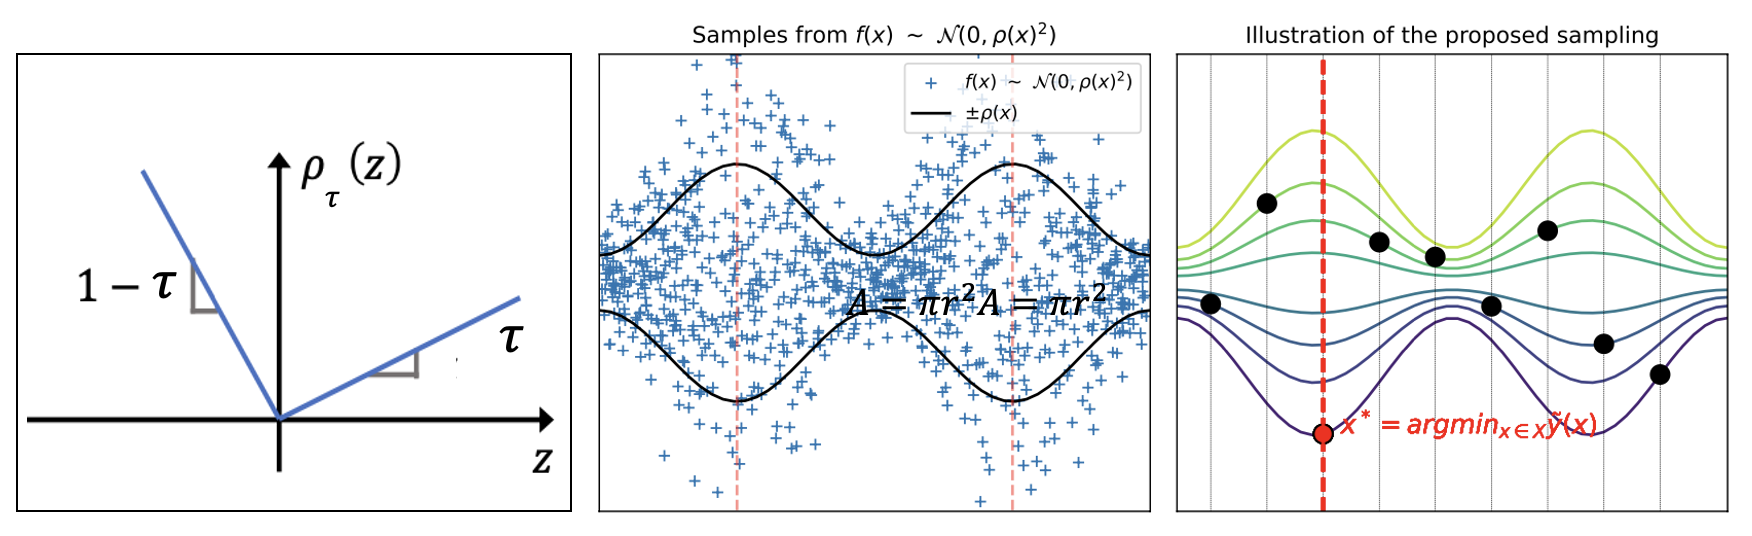
\includegraphics[scale=0.56]{pinball_loss_and_CQR}
		\refstepcounter{figure}
   		\addcontentsline{lof}{figure}{Figure~\thefigure: Pinball loss and CQR within Bayesian optimization}
		\label{fig:CQR}
		{\small \textit{Figure \ref{fig:CQR}:} in the left is a visualization of the Pinball loss function, where $z=y - \hat{y}$ \cite{romano2019conformalized}; the middle displays samples from a synthetic heteroskedasticity function and the right illustrates the sampling procedure based on $|q| = 8$ predicted quantiles \cite{salinas2023optimizing}.
		}
	\end{figure}
	 
	 A related work is \cite{salinas2023optimizing} that employs CQR to obtain quantiles with robust coverage during hyperparameter tuning via Bayesian optimization. Specifically, the calibrated quantiles are used to select the candidate for the next search, where a set of candidates is first sampled uniformly at random, and then for each of those candidates a random quantile is simply picked and is treated as the acquisition score (Figure \ref{fig:CQR}). We follow their notation and interpretation in defining the conformity score for a quantile surrogate:  
	 
	 \begin{equation}
		E_i = \max \big\{\hat{q}_{\alpha_j}(x_i) - y_i, \; y_i - \hat{q}_{1-\alpha_j}(x_i) \big\}
	 \label{scoreCQR}
	 \end{equation}
	 
	 Note that the sign of the score is positive when the target $y_i$ is outside of the interval and negative when the target falls inside the predicted interval. This allows the conformity score to account for both overcoverage and undercoverage cases. In addition, the score amplitude always measures the distance to the closer quantile between $\hat{q}_{\alpha_j}(x_i)$ and $\hat{q}_{1-\alpha_j}(x_i)$ \cite{romano2019conformalized, salinas2023optimizing}.	 


\subsection{Conformal Prediction with Cross-validation}}
Solving a NAS problem is usually computationally expensive, as each neural architecture evaluation incurs the cost of fully training and validating the underlying model on the target dataset. Motivated by the fact that NAS based on Bayesian optimization is typically allocated with a budget of 100 to 200 trials, an additional heuristic for constructing the calibration set via cross-validation (hereafter: CrossVal-CP) is employed to avoid reducing the sample size for obtaining a holdout set as performed in SCP.

At each step, the evaluated architectures are devided at random into $K$ folds. A dedicated surrogate model is trained on $K-1$ folds, while the remaining one is used as the calibration set to calculate the conformity scores. This process is repeated for $K$ times over each individual fold. Finally, conformity scores from all calibration folds are combined to form the overall calibration set, on which the quantile is computed to determine the calibration offset. For an unseen data point, the prediction is obtained by aggregating the predictions of the $K$ trained models \cite{vovk2015cross}. This approach is formally described in Algorithm \ref{alg:CVCP}. 

\begin{algorithm}[htbp]
  \caption{Conformal Prediction with Cross-validation}
  \label{alg:CVCP}
  \begin{algorithmic}[1]
    \textbf{Input:} 
    A set of observations $\{(x_{i}, y_{i})\}_{i=1}^n$, number of folds $K$, a prediction algorithm $h(\cdot)$, a non-conformity measure $\myfunc{s(\cdot)}$, nominal mis-coverage rate $\tau$, test data $x_{n+1}$. \vskip
    \textbf{Output:} a prediction set $\mathcal{C}_{\tau}(x_{n+1})}$ that covers $y_{n+1}$ with probability $1-\tau$. \vskip
    \vspace{0.5em}
    \STATE Initialise a conformity scoring set $S=\emptyset$
    \STATE Split the observations $\{(x_{i}, y_{i})\}_{i=1}^n$ into $K$ folds at random. $I_k$ denotes the index set containing indices of samples in the $k$-th fold.
    \FOR {$k$ in 1, 2, ..., K}
		\begin{enumerate}
    		\item Train $\hat{h}_{-k}(\cdot)$ on $\{(x_{i}, y_{i}) \mid i \notin I_k\}$
    		\item Compute conformity score on the $k$-th fold $S_k=\{s((\hat{h}_{-k}(x_{i}), y_i) \mid i \in I_k\}$
    		\item $S \leftarrow{S \cup S_k}$
    	\end{enumerate}
   	\ENDFOR
	\STATE Predict $x_{n+1}$: $h(x_{n+1}) \leftarrow aggregate(\{\hat{h}_{-1}(x_{n+1}), ..., \hat{h}_{-K}(x_{n+1})\})$ 
	\STATE Return $\mathcal{C}_{\tau}(x_{n+1}) \leftarrow \{y \,|\, s((h(x_{n+1}), y) \leq q\}$, where $q$ is the $\lceil(1-\tau)(n_s+1)\rceil$-th smallest value of $S$, with $n_s = |S|$.
    \end{algorithmic}
\end{algorithm}

Note that the only distinction between SCP and CrossVal-CP is how the calibration set is constructed. Since it does not place any additional restriction on the choices of the underlying surrogate, CrossVal-CP can be applied in conjunction with either ensemble predictor or quantile regressor in the same way as SCP. See Section \ref{sec:scp} for detailed configurations.

\subsection{Conformal Prediction with Bootstrapping}
Inspired by the fact that BANANAS is built on an ensemble surrogate, we further explore incorporating Jackknife+-after-boostrap \cite{kim2020predictive}, a wrapper for predictive inference designed specifically for use with ensemble learners, into the calibration step. This approach is referred as Bootstrap-CP in the following sections.

In contrast to fitting $m$ neural networks on the same training data with different random weights initializations, as applied in the BANANAS framework, a different technique to build an ensemble model is via bootstrapping. Specifically, the ensemble method starts by creating multiple training datasets by resampling the available data points with replacement. In the next step, multiple models are trained on each of the bootstrapped subsets, and their predictions are aggregated to produce the single final prediction \cite{breiman96}. The technique offers more accurate and stable estimates than a single model and has shown superior performance in application.

Jackknife+ is a type of CP algorithm that is closely related to the leave-one-out (LOO) method \cite{barber2020jackknife}. Given a set of observations $\{(x_{i}, y_{i})\}_{i=1}^n$, the idea is to fit an LOO estimator $\hat{h}_{/i}$ using all available data except for the $i$-th sample. Then, the predictive interval around the $i$-th point is obtained by offsetting the prediction from $\hat{h}_{/i}$ with the quantile of all LOO conformity scores.  Equivalently, Jackknife+ can be viewed as a special case of CrossVal-CP when the number of folds is exactly set to $K=n$.

Jackknife+-after-boostrap \cite{kim2020predictive} integrates both approaches and provides a cost-efficient wrapper by leveraging only the available bootstrapped sets and their corresponding fitted models, thereby avoid retraining ensembles on each individual bootstrapped sample. \cite{pmlr-v139-xu21h} extends this method to online setting and proves its efficiency. Compared to the CP algorithms described in earlier sections, Bootstrap-CP requires no data splitting as bootstrap ensemble is trained on random subsets from the full data. 

Implementation of Bootstrap-CP is outlined in Algorithm \ref{alg:BtCP}. In particular, if a data point appears in all bootstrapped samples, it is then excluded from the computation of conformity scores since it has no associated LOO estimator. Besides, Bootstrap-CP is only applied with the ensemble model. In summary, the BANANAS-CP framework is finally evaluated under five various predictor+CP configurations.

\begin{algorithm}[t]
  \caption{Conformal Prediction with Bootstrapping}
  \label{alg:BtCP}
  \begin{algorithmic}[1]
    \textbf{Input:} 
    A set of observations $\{(x_{i}, y_{i})\}_{i=1}^n$, number of bootstraps $B$, a prediction algorithm $h(\cdot)$, a non-conformity measure $\myfunc{s(\cdot)}$, nominal mis-coverage rate $\tau$, test data $x_{n+1}$. \vskip
    \textbf{Output:} a prediction set $\mathcal{C}_{\tau}(x_{n+1})}$ that covers $y_{n+1}$ with probability $1-\tau$. \vskip
    \vspace{0.5em}
    \STATE Initialise a conformity scoring set $S=\emptyset$
    \STATE Sample all available data with replacement and create $B$ subsets. $I_b$ denotes the indices of data points included in the $b$-th sample.
    \FOR {$b$ in 1, 2, ..., B}
		\begin{enumerate}
    		\item Train $\hat{h}_{-k}(\cdot)$ on $\{(x_{i}, y_{i}) \mid i \notin I_k\}$
    		\item Compute conformity score on the $k$-th fold $S_k=\{s((\hat{h}_{-k}(x_{i}), y_i) \mid i \in I_k\}$
    		\item $S \leftarrow{S \cup S_k}$
    	\end{enumerate}
   	\ENDFOR
	\STATE Predict $x_{n+1}$: $h(x_{n+1}) \leftarrow aggregate(\{\hat{h}_{-1}(x_{n+1}), ..., \hat{h}_{-K}(x_{n+1})\})$ 
	\STATE Return $\mathcal{C}_{\tau}(x_{n+1}) \leftarrow \{y \,|\, s((h(x_{n+1}), y) \leq q\}$, where $q$ is the $\lceil(1-\tau)(n_s+1)\rceil$-th smallest value of $S$, with $n_s = |S|$.
    \end{algorithmic}
\end{algorithm}



\section{Distribution Estimation}
\label{sec:distest}
\section{Acquisition Function and Search Strategy}
\label{sec:acq}


.......
% chapter 4
\chapter{Dataset}
\label{Dataset}
To compare the performance of BANANAS--CP with the original BANANAS algorithms and assess the role of uncertainty calibration, we run experiments on the widely used benchmark dataset NAS-Bench-201.
% chapter 5
\chapter{Experiments and Results}
\section{Setup}
\section{Baseline}


% chapter 6
\chapter{Conclusion}
\label{Conclude}
This chapter presents the central findings of this work as well as their critical discussion. Finally, it highlights limitations and corresponding opportunities for further research.



% Reference
\bibliographystyle{plain}
\bibliography{references}

% Appendix
\appendix
\chapter{Additional Experimental Results}


% Declare non-Plagiarism and independent work
\backmatter
\chapter{Ehrenwörtliche Erklärung}
Ich versichere, dass ich die beiliegende Bachelor-, Master-, Seminar-, oder
Projektarbeit ohne Hilfe Dritter und ohne Benutzung anderer als der angegebenen
Quellen und in der untenstehenden Tabelle angegebenen Hilfsmittel angefertigt
und die den benutzten Quellen wörtlich oder inhaltlich entnommenen Stellen als
solche kenntlich gemacht habe. Diese Arbeit hat in gleicher oder ähnlicher Form
noch keiner Prüfungsbehörde vorgelegen. Ich bin mir bewusst, dass eine falsche
Erklärung rechtliche Folgen haben wird.

% Declare the use of AI tools.
\vspace{0.5cm}
  \textbf{Declaration of Used AI Tools} \\[.3em]
  \begin{tabularx}{\textwidth}{lXlc}
    \toprule
    Tool & Purpose & Where? & Useful? \\
    \midrule
    ChatGPT & Rephrasing & Throughout & + \\
    ChatGPT & Debugging LaTeX syntax  & Equation/Formula & + \\
    \bottomrule
  \end{tabularx}
\end{center}

\vspace{2cm}
\noindent Unterschrift\\
\noindent Mannheim, den 31.07.2025 \hfill

\end{document}
